\documentclass[border=5pt]{standalone}
\usepackage{tikz-network}
\begin{document}
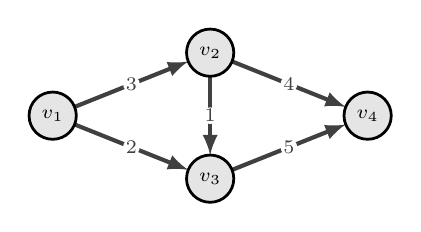
\begin{tikzpicture}
\Vertex[x=0,y=0,label=$v_1$,color=gray!20]{A}
\Vertex[x=2,y=0.8,label=$v_2$,color=gray!20]{B}
\Vertex[x=2,y=-0.8,label=$v_3$,color=gray!20]{C}
\Vertex[x=4,y=0,label=$v_4$,color=gray!20]{D}
\Edge[label=3,Direct](A)(B)
\Edge[label=2,Direct](A)(C)
\Edge[label=1,Direct](B)(C)
\Edge[label=4,Direct](B)(D)
\Edge[label=5,Direct](C)(D)
\end{tikzpicture}
\end{document}
